\newpage{}

\begin{landscape}

\hypertarget{results-per-algorithm}{%
\section{Results Per Algorithm}\label{results-per-algorithm}}

\subsection{Overview}

\begin{tabular}{lllrr}
\hline
 Algorithm   & Training on   & Estimating    &   with params &                 deviation \\
\hline
 A001        & SWEArchiv2020 & SWEArchiv2020 &         25\%P &  -1.277 $\pm$ 6.822 hours \\
 A001        & SWEArchiv2020 & SWEArchiv2020 &         50\%P &  -0.900 $\pm$ 6.369 hours \\
 A001        & SWEArchiv2020 & SWEArchiv2020 &         75\%P &   0.099 $\pm$ 6.097 hours \\
 A001        & SWEArchiv2020 & SWEArchiv2020 &         80\%P &   0.453 $\pm$ 5.573 hours \\
 A001        & SWEArchiv2020 & SWEArchiv2020 &         90\%P &   2.057 $\pm$ 5.626 hours \\
 A001        & SWEArchiv2020 & SWEArchiv2020 &        100\%P &  -1.829 $\pm$ 7.691 hours \\
 A001        & SWEArchiv2020 & SWEArchiv2021 &         25\%P & -1.546 $\pm$ 12.133 hours \\
 A001        & SWEArchiv2020 & SWEArchiv2021 &         50\%P & -1.320 $\pm$ 12.129 hours \\
 A001        & SWEArchiv2020 & SWEArchiv2021 &         75\%P & -0.675 $\pm$ 12.127 hours \\
 A001        & SWEArchiv2020 & SWEArchiv2021 &         80\%P & -0.345 $\pm$ 12.195 hours \\
 A001        & SWEArchiv2020 & SWEArchiv2021 &         90\%P &  0.805 $\pm$ 12.232 hours \\
 A001        & SWEArchiv2020 & SWEArchiv2021 &        100\%P & -1.744 $\pm$ 12.136 hours \\
 A002\_1     & SWEArchiv2020 & SWEArchiv2020 &               &  -0.000 $\pm$ 7.691 hours \\
 A002\_1     & SWEArchiv2020 & SWEArchiv2021 &               &  0.085 $\pm$ 12.136 hours \\
 A002\_2     & SWEArchiv2020 & SWEArchiv2021 &        L75\%M &  -0.326 $\pm$ 7.691 hours \\
 A002\_2     & SWEArchiv2020 & SWEArchiv2021 &        L85\%M &   0.188 $\pm$ 7.691 hours \\
 A002\_2     & SWEArchiv2020 & SWEArchiv2021 &        L95\%M &   0.214 $\pm$ 7.691 hours \\
\hline
\end{tabular}

\end{landscape}

\subsection{Fehlerverteilung in Aufgaben mit <=40 Stunden}

In der Betrachtung der im Moment zur Verfügung stehenden Daten (SWE*-Datensätze) fällt auf, dass
wir in einem bestimmten Bereich viele Aufgaben haben und im oberen Bereich vor allem Ausreißer. 

Das kann eine direkte Folge davon sein, dass nur sehr sehr wenige Aufgaben im Bereich der hohen Dauern 
vorliegen. Folglich sieht man hier in den Boxplots, dass in den höheren Dauer-Bereichen meist nur ein Mittelwert
vorliegt. Es gibt also in diesem Bereich nur einen Messwert. 

Das wiederum bedeutet, dass die Analyse der Aufgaben mit großer Dauer wenig Sinn ergibt. Wir haben hier
schlicht zu wenige Daten.

\newpage
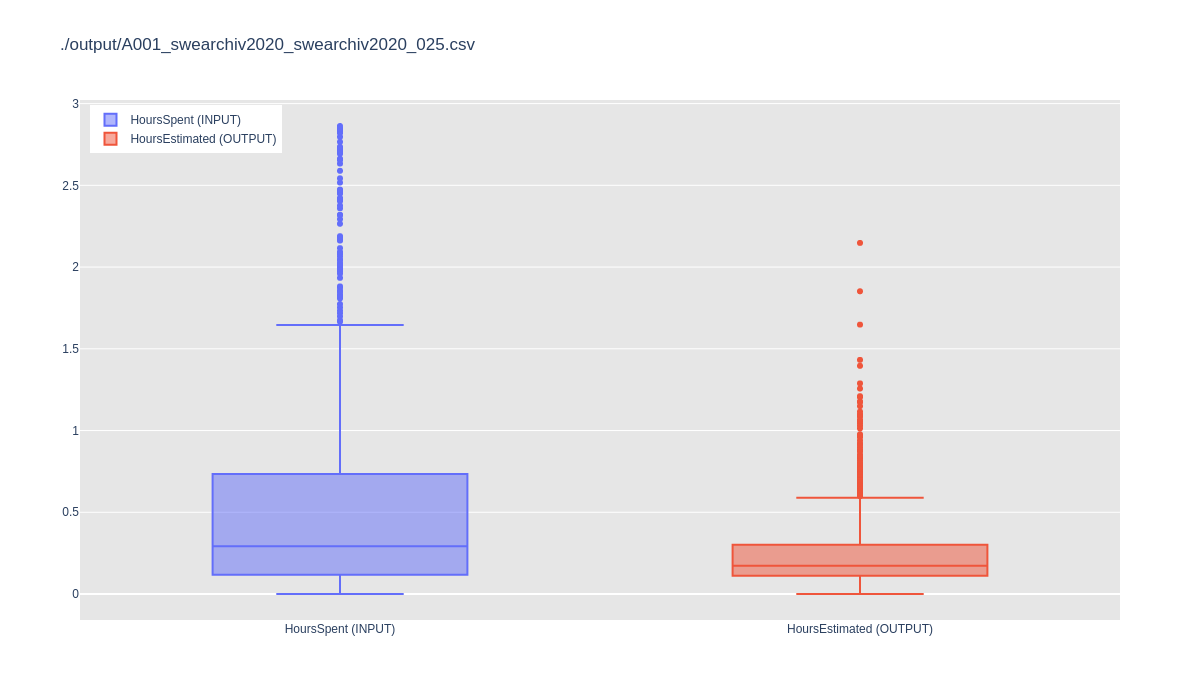
\includegraphics[width=\textwidth]{Scripts/output/A001_swearchiv2020_swearchiv2020_025.csv.png}
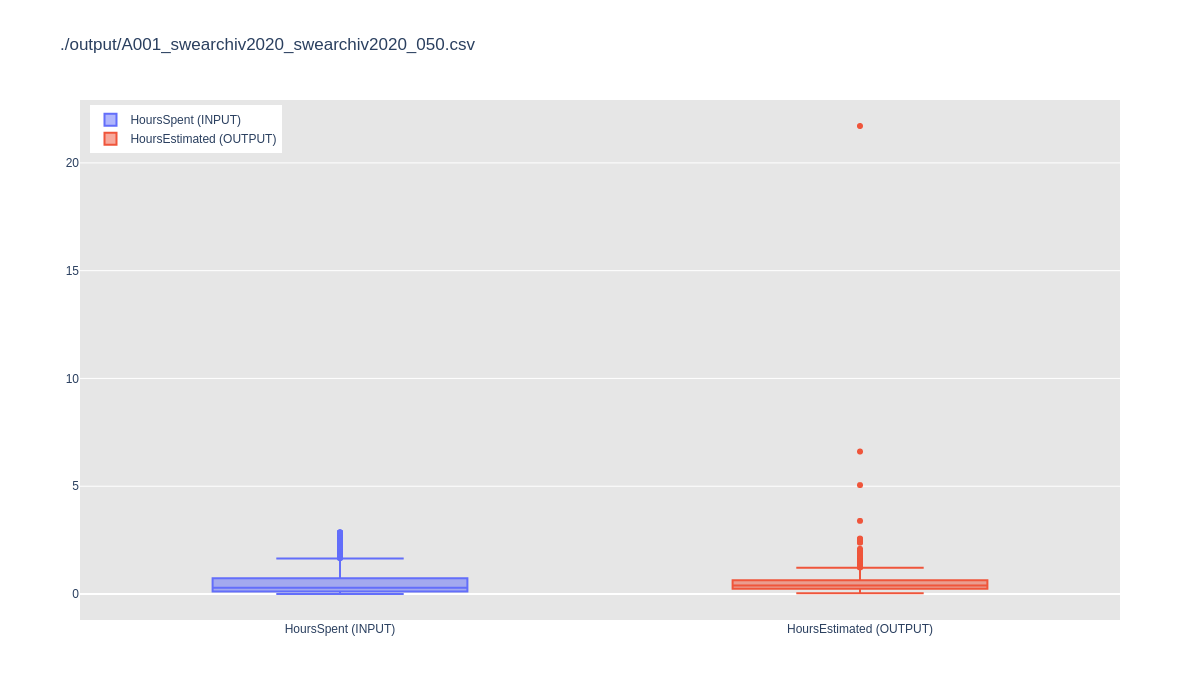
\includegraphics[width=\textwidth]{Scripts/output/A001_swearchiv2020_swearchiv2020_050.csv.png}
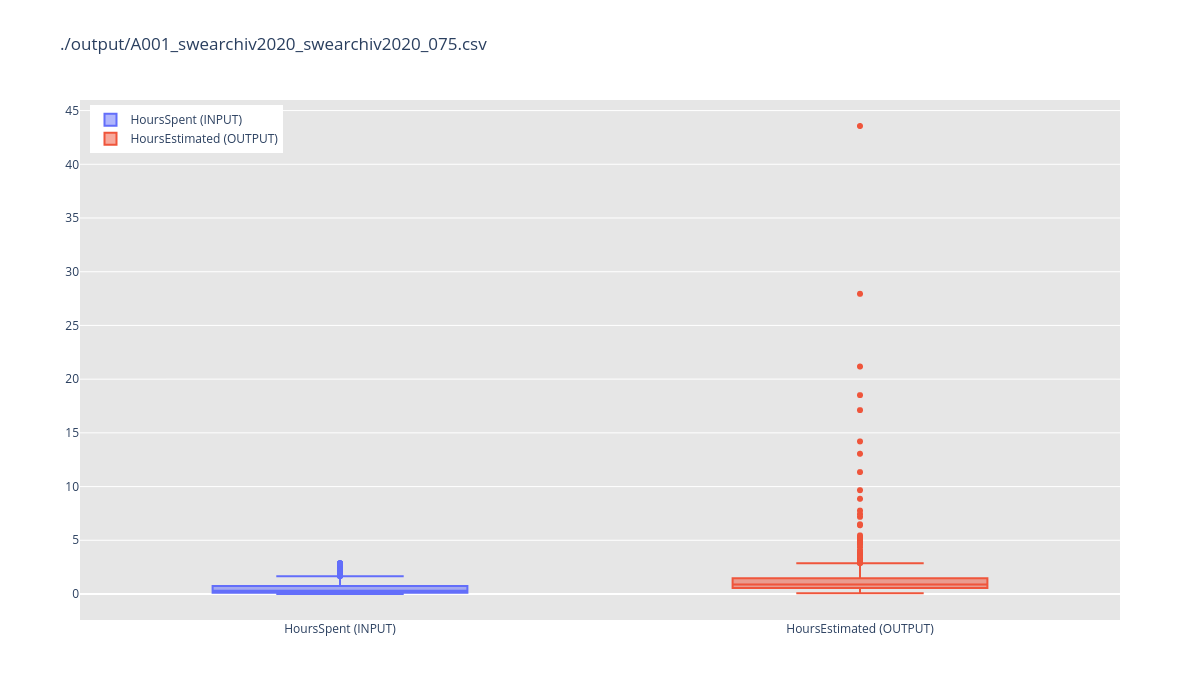
\includegraphics[width=\textwidth]{Scripts/output/A001_swearchiv2020_swearchiv2020_075.csv.png}
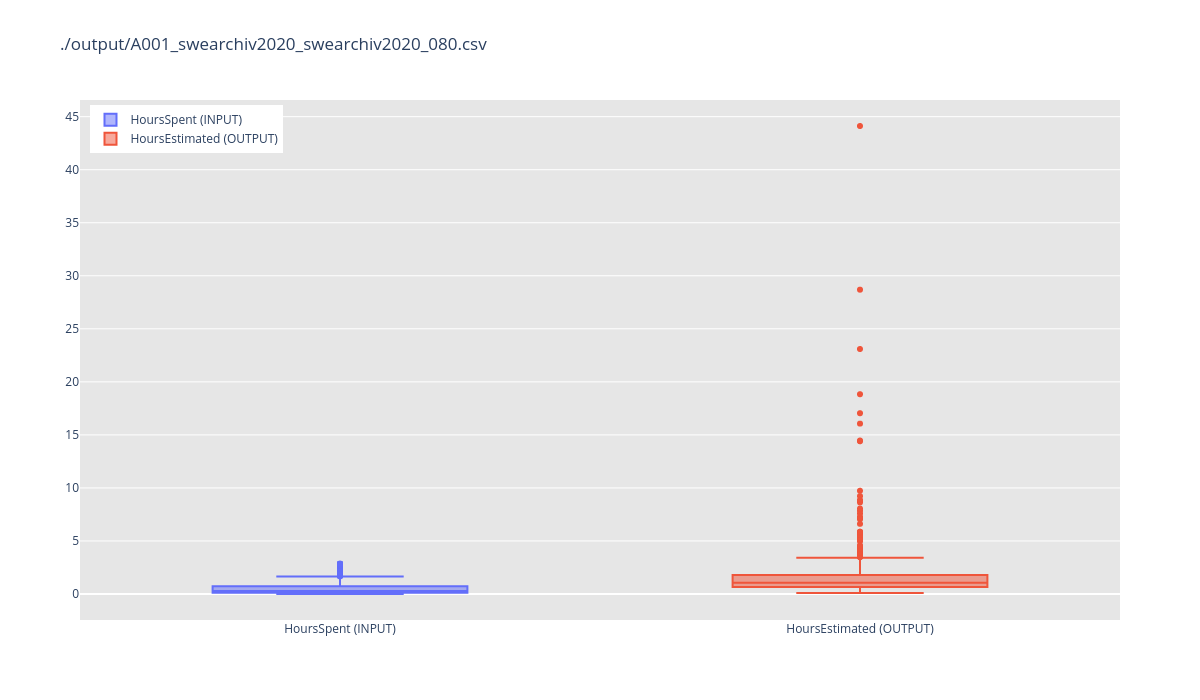
\includegraphics[width=\textwidth]{Scripts/output/A001_swearchiv2020_swearchiv2020_080.csv.png}
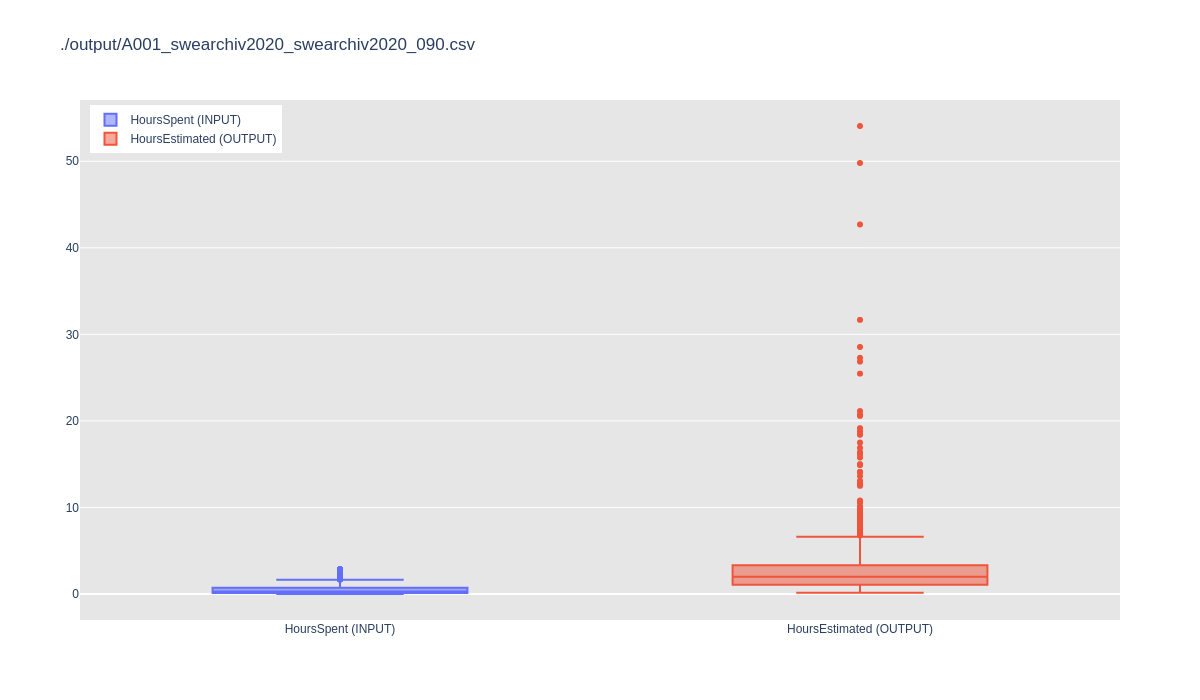
\includegraphics[width=\textwidth]{Scripts/output/A001_swearchiv2020_swearchiv2020_090.csv.png}
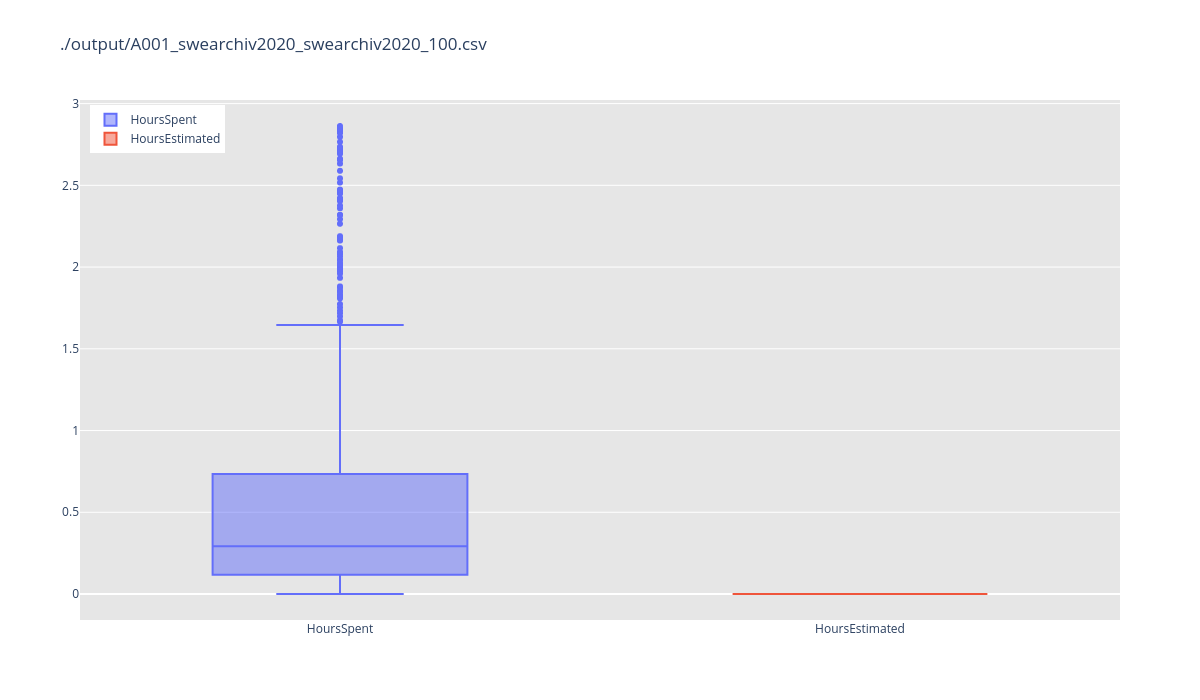
\includegraphics[width=\textwidth]{Scripts/output/A001_swearchiv2020_swearchiv2020_100.csv.png}
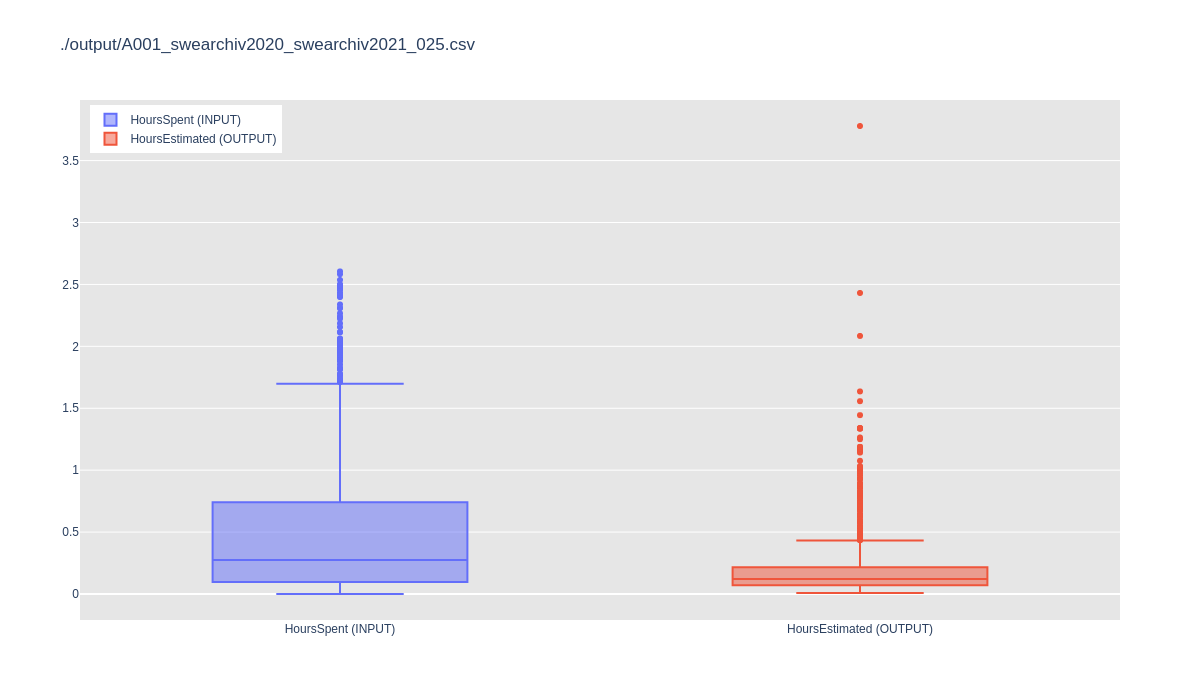
\includegraphics[width=\textwidth]{Scripts/output/A001_swearchiv2020_swearchiv2021_025.csv.png}
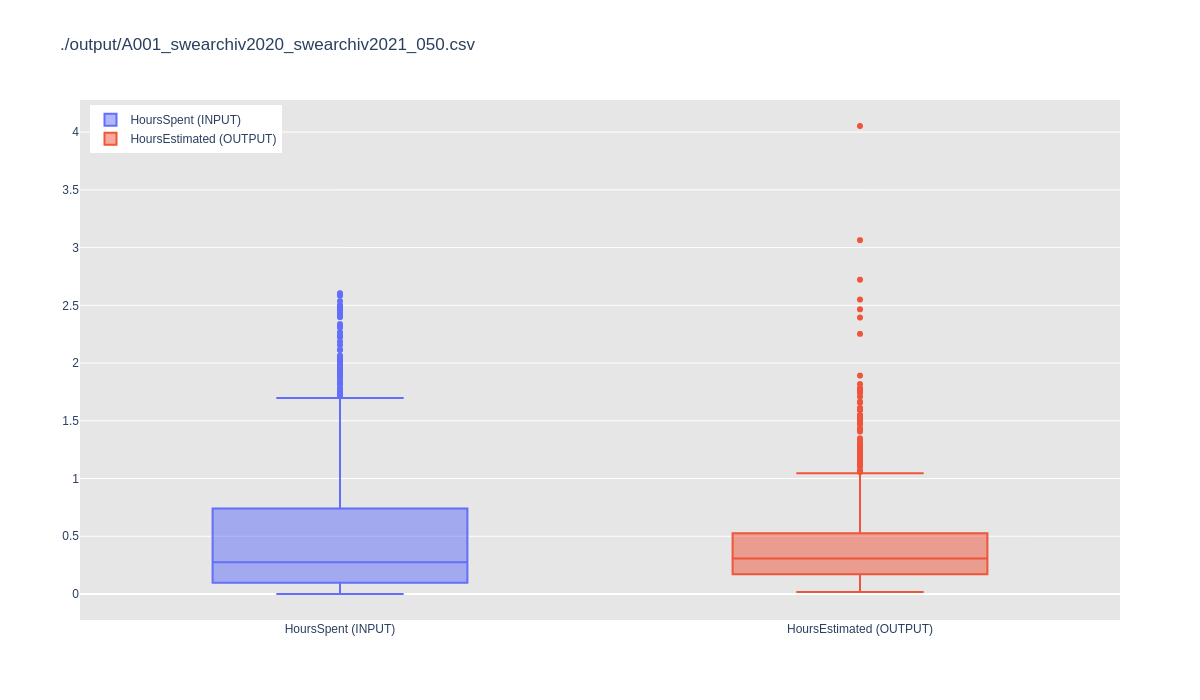
\includegraphics[width=\textwidth]{Scripts/output/A001_swearchiv2020_swearchiv2021_050.csv.png}
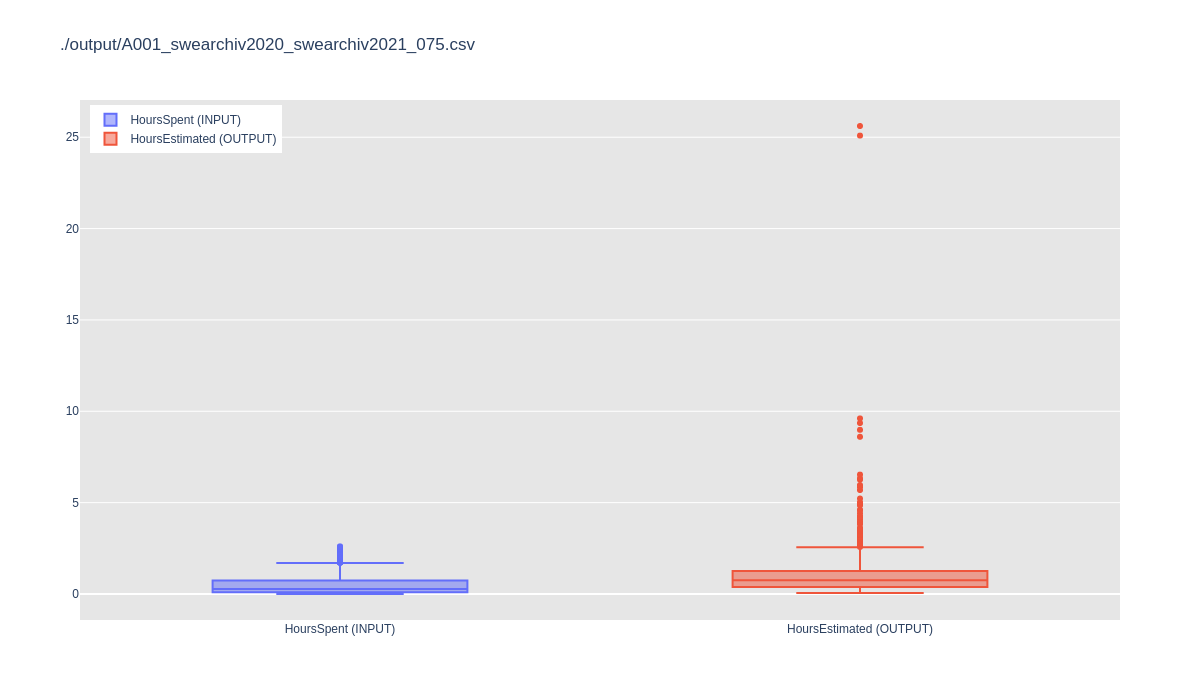
\includegraphics[width=\textwidth]{Scripts/output/A001_swearchiv2020_swearchiv2021_075.csv.png}
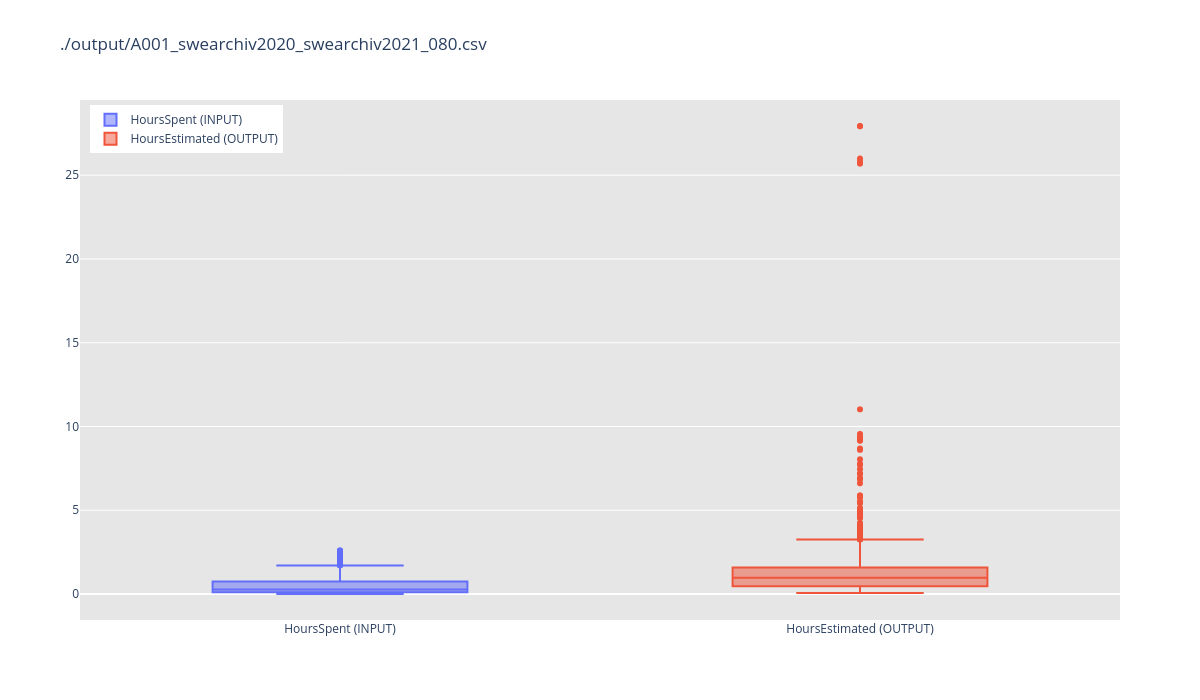
\includegraphics[width=\textwidth]{Scripts/output/A001_swearchiv2020_swearchiv2021_080.csv.png}
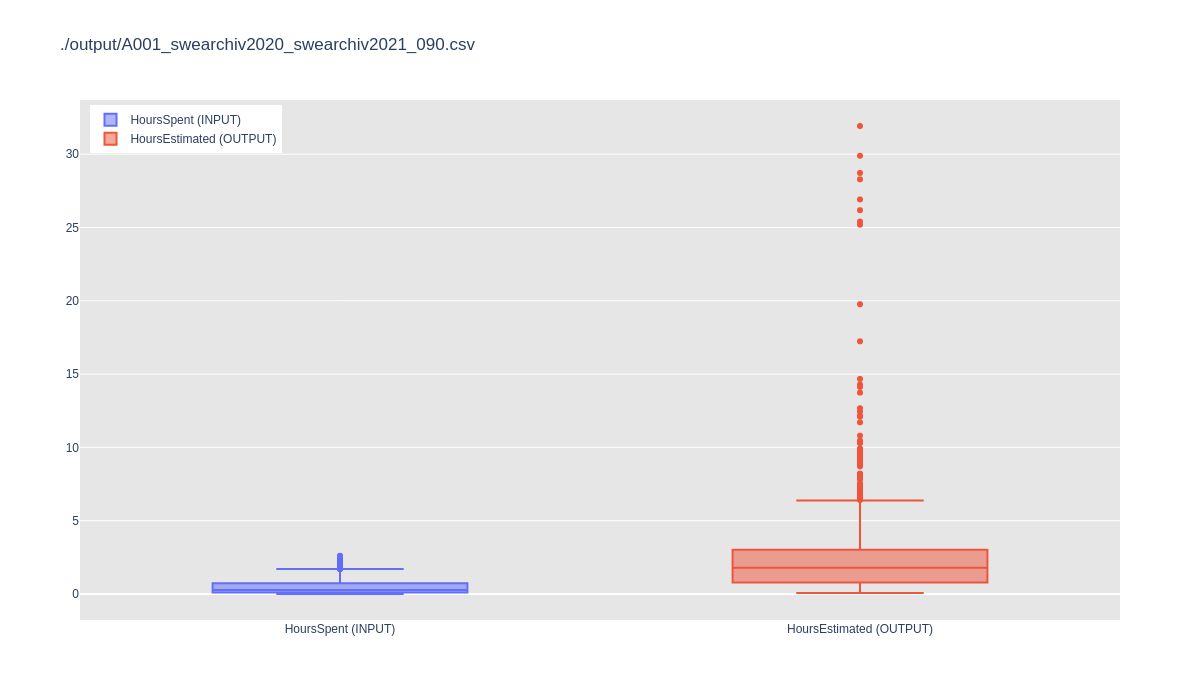
\includegraphics[width=\textwidth]{Scripts/output/A001_swearchiv2020_swearchiv2021_090.csv.png}
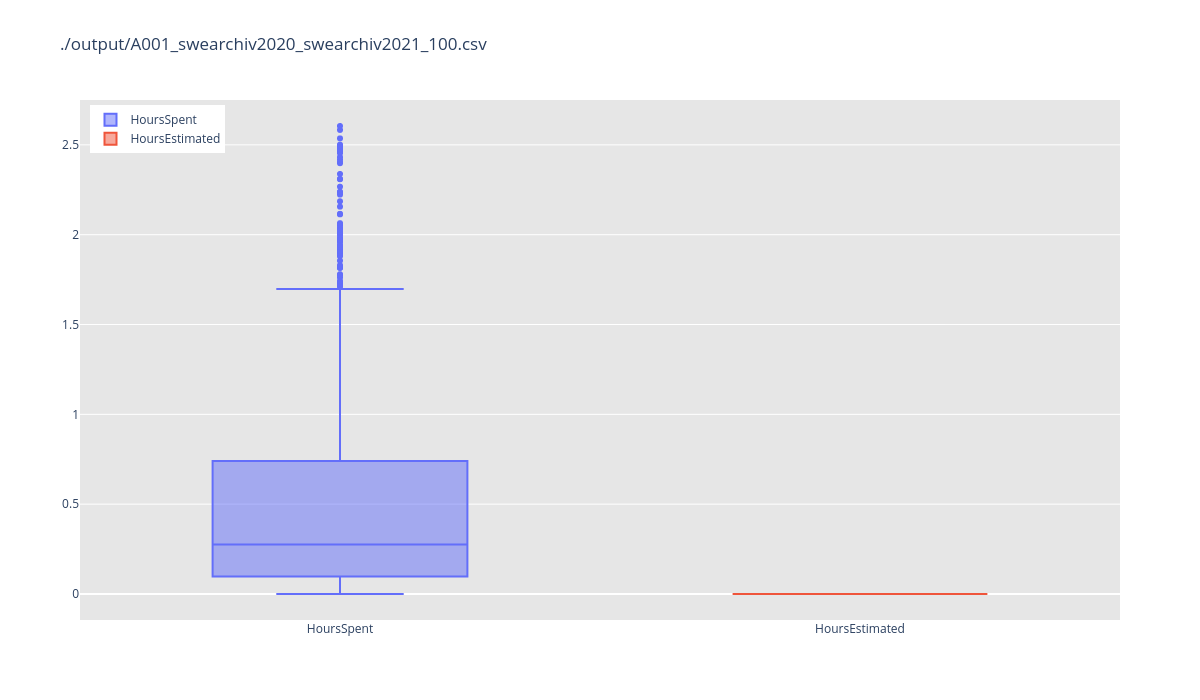
\includegraphics[width=\textwidth]{Scripts/output/A001_swearchiv2020_swearchiv2021_100.csv.png}


